\documentclass[a4paper,10pt]{article}
\usepackage[utf8]{inputenc}
\usepackage[french] {babel}
\usepackage[T1]{fontenc}
\usepackage{lmodern}
\usepackage{graphicx}
\usepackage{graphics}
\usepackage{ulem}
\usepackage{amssymb}
\usepackage{url}
\usepackage{circuitikz}
\usepackage{subfig}
\usepackage[a4paper]{geometry}
\geometry{hscale=0.7,vscale=0.7,centering}
\usepackage{vmargin}
\usepackage{amsmath}
\usepackage{amssymb}
\usepackage{amsthm}
\usepackage{moreverb}
\usepackage{listings}
\usepackage{qtree}
\graphicspath{{IMAGES/}}
\newtheorem{theorem}{Théorème}[section]
\newtheorem{defi}{Définition}[section]
\newtheorem{propri}{Propriété}[section]
\newtheorem{ex}{Exemple}[section]
\newtheorem{thesis}{Thèse}[section]
\newtheorem{cor}{Corollaire}[section]

\usepackage{color}

\definecolor{gris}{rgb}{0.95,0.95,0.95}


% Param�rage des listings
\lstset{basicstyle=\footnotesize\ttfamily}
\lstset{keywordstyle=\color[rgb]{0,0,1}\bfseries}
\lstset{identifierstyle=\color{black}}
\lstset{commentstyle=\color[rgb]{0,0.4,0}}
\lstset{stringstyle=\color[rgb]{0.7,0,0}}
\lstset{showstringspaces=false}
\lstset{showtabs=false}
\lstset{tabsize=3}
\lstset{extendedchars=true}
\lstset{breaklines=true}
\lstset{postbreak={}}
\lstset{breakautoindent=true}
\lstset{breakindent=0pt}
\lstset{xleftmargin=0.1cm}
\lstset{xrightmargin=0cm}
\lstset{frame=tb,rulecolor=\color[gray]{.4}}
\lstset{captionpos=b}
\lstset{aboveskip=0.5cm,belowskip=0.5cm}
\lstset{numbers=left}
\lstset{columns=fixed}
\lstset{language=java}



\newcommand{\code}[1]{\lstinline{#1}}

\setlength{\parskip}{.7em}

\begin{document}


\begin{flushleft}

\includegraphics[scale=0.3]{logo_ist.jpeg}
\end{flushleft}


\vspace{1cm}

\begin{center}{
\scshape{\LARGE Wolves and squirrel : Part 1 }}

\vspace{0.5cm}
\hbox{\raisebox{0.4em}{\vrule depth 0pt height 0.05cm width 16cm}}
{\setlength{\parskip}{0.2cm}

 \Huge
 \bfseries
 \LARGE  Parallel and Distributed Computing
 \\
CPD \\

\vspace{0.2cm}

}
\vspace{0.5cm}

\hbox{\raisebox{0.4em}{\vrule depth 0pt height 0.05cm width 16cm}}
\vspace{2.5cm}


\end{center}

\vspace{3cm}


\vfill
\begin{flushright}
\textbf{Group 30 :}\\
Cappart Quentin (77827)\\

\end{flushright}
\newpage

\setcounter{page}{1}

\renewcommand\thepage{\arabic{page}}


\newpage

\section*{Decomposition done}

\section*{Conflict resolution}

The conflict resolution is done by the architecture of the serial version. Indeed, all the conflicting movement are not made
directly but their are kept in memory and proceeded after each subgeneration with the \texttt{update} method.
So, with the parallelization, given that we have an implicit synchronization after each iteration of the main loop (generation loop),
the conflict are implicitly resolved.

\section*{Performances analyze}

The following array recaps the execution time of the OMP version with severals numbers of threads.
\begin{table}[!ht]
\centering
\begin{tabular}{|r||r|r|r|r|}
  \hline
    Instance     & 1 thread   & 2 threads   & 4 threads  & 8 threads  \\
  \hline
    ex3.in       &  0.008     & 0.008        & 0.017       &  0.020 \\ 
  \hline
    world\_10.in &  0.011      &  0.006       & 0.021       & 0.035 \\ 
  \hline
   world\_100.in &  0.111      & 0.070        & 0.068      & 0.1278 \\ 
  \hline
  world\_1000.in &  12.885   & 7.712       & 6.534      &  6.522 \\ 
  \hline
\end{tabular}
\caption{Performances (in sec) for the different instances.}
\end{table}

We did these experiments on a computer with 4 cores with the input \texttt{instance 10 9 8 100}. We
let to the "iteration print" in the code\footnote{If we remove it, the execution time is to fast to do an useful analyze.}.
First, we notice that for the smallest instance, \texttt{ex3.in},
more we have threads, more the program is slow. This is normal. Indeed, given that the instance are small, the overhead of the threads (creation, repartition and
synchronization for example), surpass the gain that we have by the multithreading.
For the instance \texttt{world\_10.in}, we notice it from 4 threads.
For the biggest instance, \texttt{world\_1000.in}, we see the speedup with severals threads. The speedup decreases with the number
of thread\footnote{We gain more from 1 to 2 threads than for 2 to 4 threads.}.
A last comment is that, given that the computer has 4 cores, we loose the interest of multithreading after 4 threads.
\\

Now, let's compare the execution time for  world\_1000.in with the ideal speedup\footnote{$S = \frac{T_{serial}}{N_{threads}}$}
with different numbers of threads :

\begin{figure}[!ht]
  \centering
  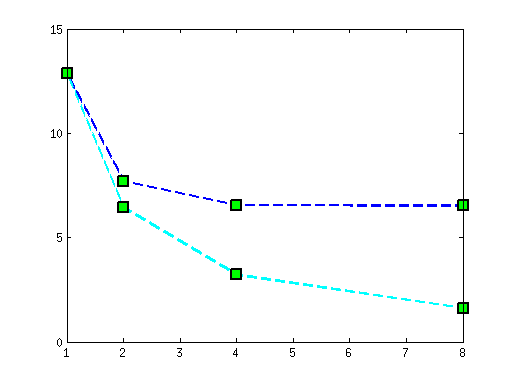
\includegraphics[width=8cm]{speedup.png}
  \caption{Comparison with the ideal speedup.}
\end{figure} 

We two threads we are relatively close to the ideal speedup. However the gap grows with more threads. We expected this king of results.
Indeed, there is always overhead when we deal with threads and all of our code is not multithreaded, so it's normal that we don't reach
the ideal result.
\end{document}

